\documentclass[../EBEXPaper2.tex]{subfiles}
\begin{document}
%------------------------------------------------- 
\section{Detector Readout}
\label{sec:detector_readout}

% frequency domain multiplexing
The \ac{TES} bolometers were biased with constant voltage~\citep{lee_appliedoptics_1998}.
Incident optical power fluctuations modulated the current across the bolometer and across a series inductor and capacitor.
A \ac{SQUID} transimpedance pre-amplifier converted the modulated current to a voltage signal that was subsequently further amplified, digitized, and filtered~\citep{yoon_apl_2001}.

We used \ac{FDM} to couple several detectors to a bias and a readout line~\citep{yoon_apl_2001}.
When the \ac{EBEX} program began power dissipation of state-of-the-art analog \ac{FDM} readout boards consumed approximately 5~W per readout channel, a prohibitive level for a balloon-borne payload.
We have therefore embarked on implementing the new \ac{DfMUX} scheme that had approximately $\times$10 lower power consumption per readout channel~\citep{dobbs_ieee_2008}.
\ac{EBEX} was the first experiment to implement this scheme multiplexing 8 detectors with two wires in its 2009 engineering flight, and the first to multiplex 16 detectors in its \ac{EBEX2013} flight. 

The \ac{EBEX} readout system required investment of effort along three dimensions:  development and testing of the new \ac{DfMUX} electronic boards, the development of automated on-board software to bias and read the \ac{TES} bolometers and the \ac{SQUID} pre-amplifiers, and the development and implementation of a cooling system that dissipated the $\sim$\PinBRC~W dissipated by the \ac{DfMUX} boards.
We discuss only the first element in this section.
The software and cooling system are discussed in \ac{EP3}.   
\citet{Aubin_TESReadout2010}, \citet{MacDermid_SPIE2014}, \citet{MacDermid_thesis}, and \citet{aubin_thesis} give more details about the \ac{EBEX} readout system. 

\subsection{Microstrips} 

To transmit signals electrically from LC boards to \ac{SQUID} amplifiers, wiring assemblies called microstrips were designed and constructed.
Operating on the transistion edge of the superconducting state, the \ac{TES}s have an internal resistance of about 1~$\Omega$ just above the transition temperature.
In order to measure the changes in the resistance of the \ac{TES}s, the rest of the readout pipeline prior to amplification requires superconducting wiring to avoid dominating the \ac{TES} resistance with other stray resistances~\citep{dobbs_revSciInst_2012}.
The wiring in the microstrips consists of flattened NbTi wire with a critical temperature of 9.2~K, well above the temperature of the LHe stage in which it is mounted.
NbTi also has relatively low thermal conductivity for a superconducting material which reduces the conductive load on the sub-kelvin stages from the microstrips.

The microstrip geometry was chosen due to the details of the digital frequency-domain multiplexing readout.
Since signals for separate detectors are measured in the frequency-domain, stray inductance in the readout wiring reduces the effective voltage bias at the detectors and widen the RLC bandpass for each detector increasing crosstalk.
To minimize the stray inductance, the parallel-plate waveguide (PPW) geometry was chosen over more traditional geometry such as twisted pairs, which has inductances on order $4-8\ \frac{\mathrm{nH}}{\mathrm{cm}}$.
Since the length of microstrips needs to be $70-95$~cm, this would give inductances as high as 760~nH, which is not negligible compared to the 24~$\mu$H inductance values used in the LC circuitry for setting the detector resonances. % 13-22 uH before

Since NbTi has a very low solderability, the flat NbTi wire is fabricated from $0.191$~mm diameter NbTi wire that is copper-clad with total diameter of $0.305$~mm, supplied by Supercon, Inc., and rolled flat to thickness of about 33~$\mu$m.
The flattening of the wires was performed by the H Cross Company.
Since the copper is significantly softer than the NbTi, the final cross-sectional dimensions of the NbTi are 762 by 33~$\mu$m as the copper migrates to the edges of the flattened material during the rolling process.
The copper-cladding is dissolved from the entire length of the flattened wire except for the ends using a nitric acid wash.
The copper-cladding on the ends remains to allow soldering of the wire to connectors.

The microstrips each consist of 8 pairs of flattened NbTi wire, and with the x16 multiplexing scheme used in the detector readout, each microstrip carries the signal from 128 detectors.
To isolate the two wires in each pair, a film of $7.6$ $\mu$m thick Kapton HN is used as a spacing layer.
Adjacent pairs are spaced apart by $940$ $\mu$m and are secured in their position by a layer of $64$ $\mu$m thick Kapton HN tape with silicone adhesive.
The overall construction is shown in Figure \ref{fig:ustrip}. %This geometry is called a parallel-plate waveguide, however, due to initial convention, it will still be referred to as a microstrip. %Details for the construction of the microstrips can be found in \cite{polsgrove09}.

\begin{figure}[t]
  \centering
    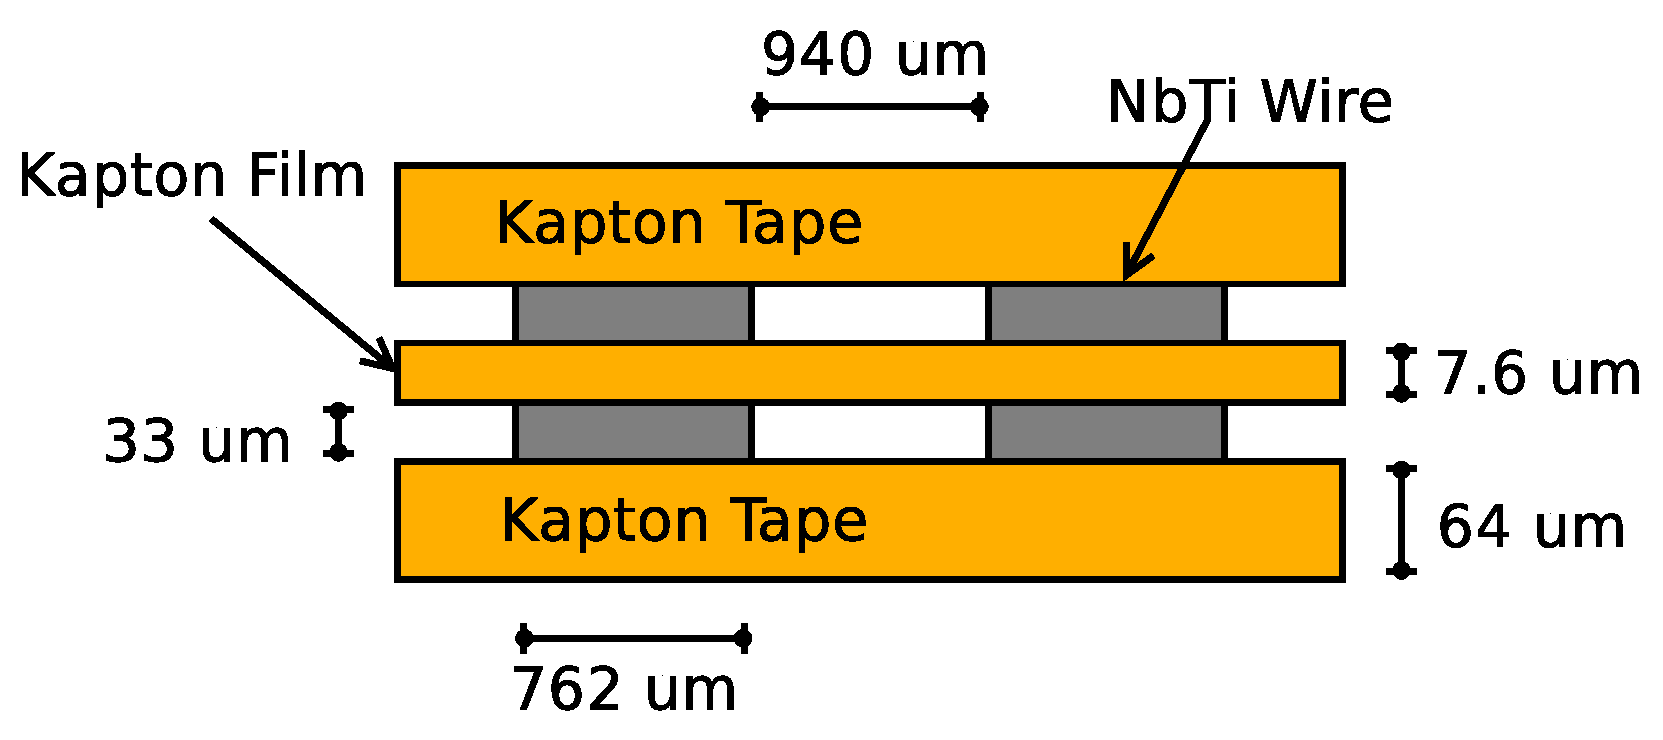
\includegraphics[width=0.45\textwidth]{./images/ustrip}
    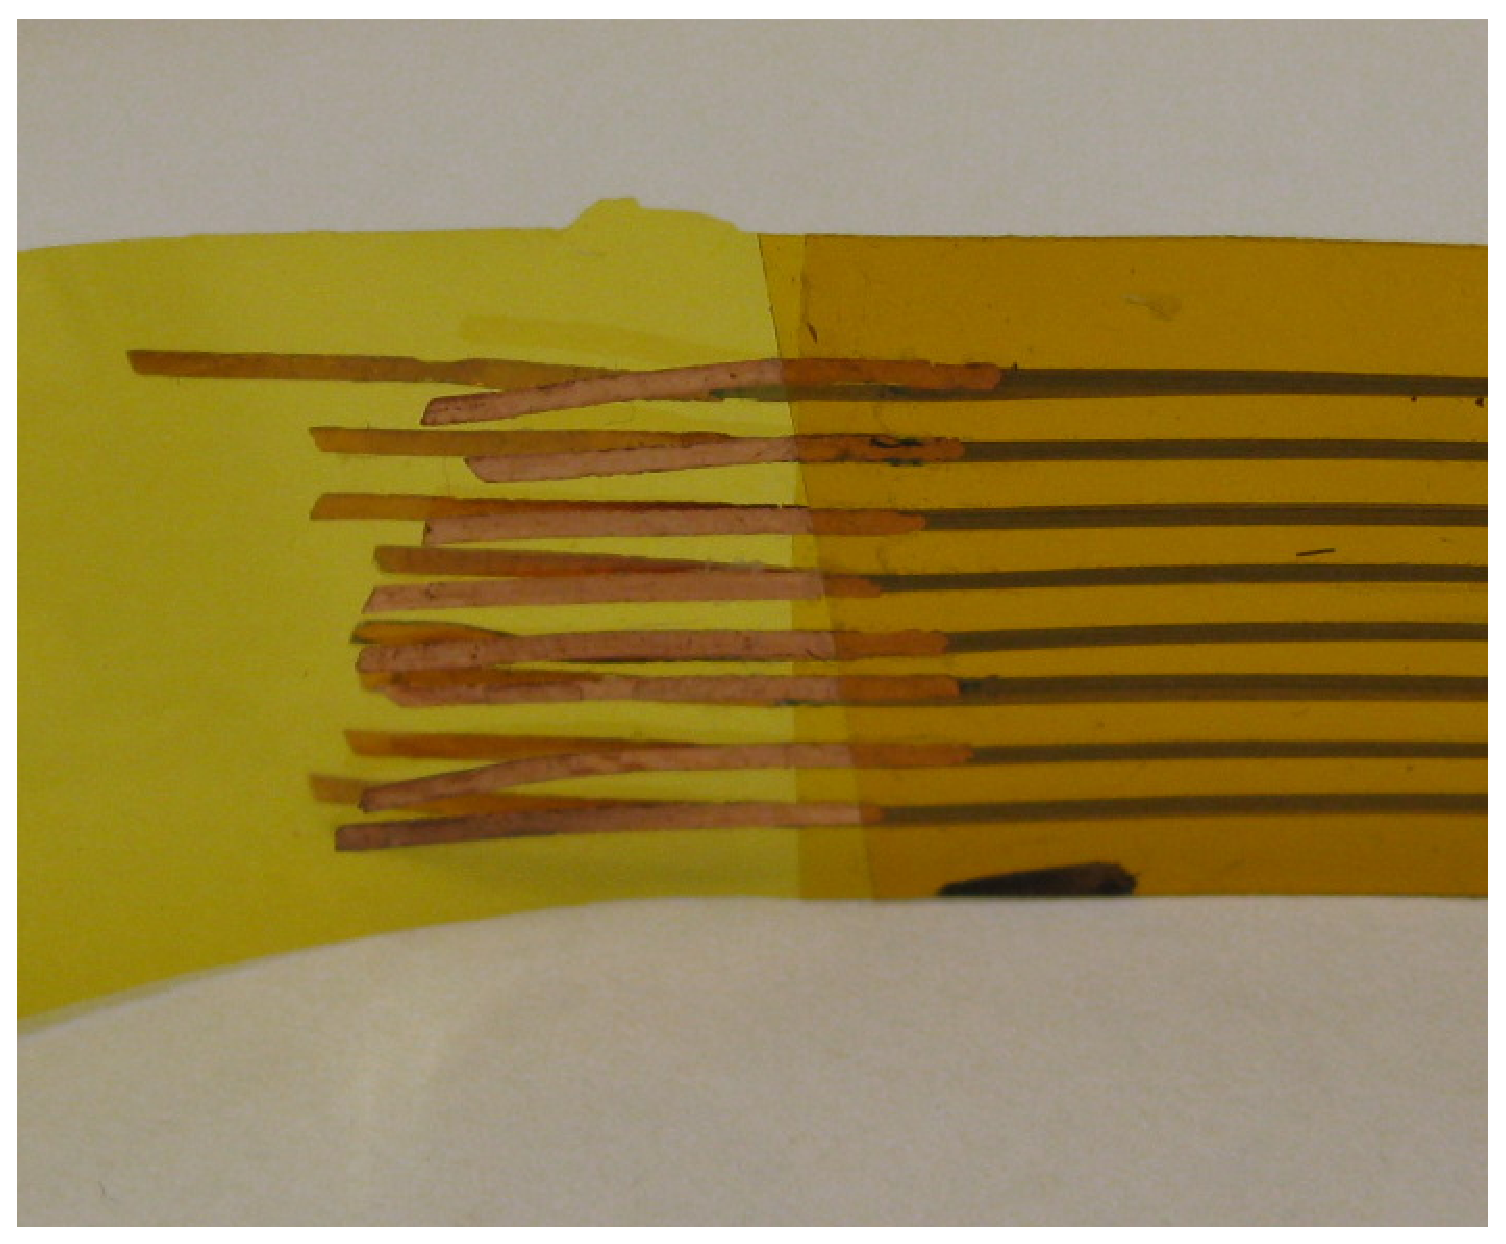
\includegraphics[width=0.3\textwidth]{./images/ustrip_end}
    \includegraphics[width=0.35\textwidth]{./images/ustrip_done}
  \caption{Diagram of the microstrip geometry (upper left panel), image of copper-clad NbTi wire ends (upper right panel), and image of the microstrip soldered to Micro-D connectors (lower panel).}
  \label{fig:ustrip}
\end{figure}

The ends of the flattened wires in each microstrip are soldered to small flexible circuit board attached to a micro-D connector on each end.
The ends of the microstrip can then be mated to corresponding connectors from the LC boards and on the \ac{SQUID} amplifier boards.

\ac{EBEX} instrument microstrips are expected to have inductances of $24.5$ and $33.3$ nH for the $700$ and $950$ mm microstrips, respectively. These values are suitably small compared to the resonance defining inductances to have a negligible affect on the resonance frequencies and detector response.

The microstrips pass through the interior of the RF towers with a single cable assembly running temperature sensor signals from the focal planes to electronics at the cold plate.
To reduce conductive loading, each cable assembly is thermally connected to each of the joints between thermal isolation segments, which are then kept at 330 mK and 0.9 K by connections to the adsorption refrigerators.
The RF towers prevent RF pickup by the microstrips and are described in \ac{EP1}.

%The geometry described above was chosen in the design of the microstrips due to the details of the digital frequency-domain multiplexing readout. Since signals for separate detectors are measured in the frequency-domain, stray inductance in the readout wiring can shift the resonance frequencies for detectors as well as reduce response due to the stray impedance in the wiring. To minimize the stray inductance, the PPW geometry was chosen over more traditional geometry such as twisted pair geometry, which has inductances on order $4-8\ \frac{\mathrm{nH}}{\mathrm{cm}}$. Given the length of microstrips needs to be $700-950$ mm, this would give inductances as high as 760 nH, which is not negligible compared to the $13-22\ \mu$H indutance values used in the LC circuitry for setting the detector resonances. %For parallel, perfectly conducting wires of constant arbitrary geometry, the capacitance and inductance per length are related as,
%\begin{equation}\label{eq:genLCperlength}
%  \mu\epsilon = \frac{L}{l}\frac{C}{l}
%\end{equation}
%For PPW geometry, assuming small separation of the wires compared to their widths, the inductance per length is then,
%\begin{equation}\label{eq:indlength}
%  \frac{L}{l} = \mu\epsilon \frac{h}{\epsilon w} = \mu \frac{h}{w}
%\end{equation}
%for $\mu$ and $\epsilon$ of the medium between the wires which are separated by $h$ and have width $w$. The relative permeability of Kapton HN is very close to one and the relative permittivity is 3.5 \cite{kapton}, so the predicted inductance per length for the given geometries are $0.126$ and $0.209\ \frac{\mathrm{nH}}{\mathrm{cm}}$ for the $7.6$ and $12.7$ micron films, respectively.

%Capacitance measurements were made at room temperature of one of the microstrip assemblies prior to attachment of the flexible circuit boards using an SRS720 LRC meter. The capacitance was measured across the two flattened wires of each pair in the microstrip for 10 microstrip assemblies and the inductances calculated, however, the measured values were a factor of 3 higher than the predicted $0.209\ \frac{\mathrm{nH}}{\mathrm{cm}}$. This can be partially attributed to an adhesive spray used in the construction process effectively increasing the separation between the wires in each pair beyond the $12.7$ micro film thickness. The microstrips still showed a improvement in inductance compared to the twisted-pair geometry. Cold measurements of the stray inductance of detector circuits using the method described in \cite{hubmayr09} showed inductances per length of $0.58\ \frac{\mathrm{nH}}{\mathrm{cm}}$ for the microstrips, in good agreement with the warm measurements. 


\subsection{Digital Frequency Domain Multiplexing}
\label{sec:dfmux}

% DfMUX
A schematic of the \ac{DfMUX} is shown in Figure~\ref{fig:dfmux_schematic}.
A comb of 16 sinusoidal voltages $\sum_{i=1}^N{V_i (f_i)}$ was digitally generated by a room temperature \ac{FPGA}\footnote{Xilinx Virtex-4 \ac{FPGA}}. 
The voltages converted to analog were shunted by a $\sim$30~m$\Omega$ resistor $R_{bias}$ to provide constant voltage to 16 parallel RLC resonators in which the $\sim$1~$\Omega$ resistor $R_i$ was the \ac{TES} of the bolometer.
The $\sim$24~$\mu$H inductors L were coupled to an appropriate capacitor $C_i$ such that the resonant frequencies were between 200 and 1200~kHz. 
The currents flowing through the bolometers were summed and coupled to low-impedance 100-element series-array \ac{SQUID}~\citep{Huber2001}, referred to as a \ac{SQUID} in this paper.
The \ac{FPGA} also generated a second identical comb of 16 frequencies $-\sum_{i=1}^N{V_i(f_i)}$ converted to current by the resistor $R_{null}$ that was 180$^o$ out of phase with the first and that was summed with the bolometer currents at the \ac{SQUID} input coil to reduce the requirements on the \ac{SQUID} dynamic range.
The \ac{SQUID}s were operated in a shunt-feedback with a low-noise transistor op-amp and a feedback resistor $R_{FB}$ of 5000~$\Omega$ located on a custom \ac{SQUID} controller circuit board~\citep{lanting_thesis}.
The length of the wiring\footnote{These cables were custumly assembled by Tekdata} between the \ac{SQUID} boards and the room temperature electronics is 19.5~cm.
These cables are heat-sunk to the five temperature layer of the \ac{EBEX} cryostat to minimize the thermal load on the detector cryogenic stage.
The phase shift caused by these wires is below the 45$^o$ requirement for the feedback loop to provide proper negative feedback within the readout bandwidth~\citep{dobbs_revSciInst_2012}.
The amplified output bolometer current comb was digitized at 25~MHz by the \ac{FPGA}, demodulated with a comb of frequencies $\sum_{i=1}^N{V'(f_i)}$, and decimated to 190.73~Hz.
The data was packetized by a Microblaze virtual processor that was part of the \ac{FPGA}, and streamed to the flight control computer over Ethernet for storage.
\begin{figure}[htbp]
\begin{center}
\epsscale{0.9}
\plotone{images/detectors_and_readout/FDM2.png}
\caption{Schematic of the frequency domain readout system following~\citet{aubin_thesis}.
Colors encode different temperature stages. For the test flight $N$ was 8; for the \ac{EBEX2013} flight it was 16.
\label{fig:dfmux_schematic} }
\end{center}
\end{figure}

% \begin{figure}[htbp]
% \begin{center}
% \epsscale{0.6}
% \plotone{images/detectors_and_readout/squidBoard.eps}
% \caption{A circuit board with 8 \ac{SQUID}-arrays mounted (only 4 shown) surrounded by mu-metal Cryoperm shielding.  One 30~m$\Omega$ bias resistor per multiplexed unit is also shown.}
% \label{fig:squid_board}
% \end{center}
% \end{figure}

% In addition to its two main design constraints the implementation of a Microblaze virtual processor allowed \ac{DfMUX} to perform significant bolometer tuning, reducing the computer requirements of the flight control computer significantly.
% During the configuration of the array for sky observations it was necessary to determine first the biases for the \ac{SQUID}s, then provide and null the bias for each bolometer, and finally to step down the bolometer bias until each channel reached a fixed fraction of its initial resistance.
% Each of these steps were performed by tuning algorithms stored on flash memory on the \ac{DfMUX} boards and run (in python) on the virtual processor.
% The flight computer simply sent a JSON formatted request to the board, and stored the result, returned in the same format over Ethernet.

% Power/hardware
We operated 28 \ac{DfMUX} readout boards and 112 \ac{SQUID}s during the \ac{EBEX2013} flight.
Each \ac{DfMUX} board provided biases and read out 4 \ac{SQUID}s, and thus also provided biases to 64 detectors. 
The boards were separated into four \ac{BRC} containing either 6 or 8 boards.
In addition to the readout boards, each BRC also had a VME backplane, a clock distribution board, and an ethernet communication ring switch.\footnote{ET-9RS 9-port and SLX-10MG 10-port Ethernet ring switch}
One of the BRC also held boards that were used to cycle the sub-Kelvin refrigerators and readout receiver housekeeping temperatures. 
The clock distribution boards provided the backplane with a 25~MHz clock signal, the commands to turn on/off power to individual boards, and the commands triggering the re-programming of the boards' firmware.
Ethernet communication between the boards and the flight computer is discussed in \ac{EP3}.  
Each BRC shell acted as a Faraday cage, shielding the readout electronics from RF signals.
Two other electronic crates each populated with DC/DCs\footnote{MOR DC/DC} converted unregulated battery or solar power to regulated 24~V~\citep{sagiv_thesis, Sagiv_MGrossman2012}.
Each crate supplied \PperPcrate~W to two BRCs; this is \PperDfMUX~W per \ac{DfMUX} board or \PperCh~W per readout channel.
Factoring in the 82\% efficiency of the DC/DC the total power consumption of the readout system was \PoutBRC~W.

%on-board processing
The virtual processor of each \ac{DfMUX} board was programmed to perform tasks on up to two \ac{SQUID}s or the detectors wired to them simultaneously.
These tasks included tuning the \ac{SQUID}s, configuring the voltage biases for the detectors, and ensuring the \ac{SQUID}s were operated within their dynamic range~\citep{macdermid_aip2009}.
With this architecture we parallelized the array tuning process saving observing time and reducing the load on the flight control computer.
Since each \ac{DfMUX} board operates four \ac{SQUID}s and can perform two tasks at a time, the tuning time of the detector array is equivalent to the time to tune two \ac{SQUID}s and their detectors and is independent of the total number of detectors populating the focal plane.

The \ac{DfMUX} `algorithm manager', written in python, listened for requests issued by the flight control computer via Ethernet communication and executed the requested python coded task.
The python tasks were stored on the \ac{DfMUX} board flash memory.
Once the task was completed, the result was sent back to the flight control computer through Ethernet for storage.

The interaction between the \ac{DfMUX} boards and the flight control computer is further described in \ac{EP3}


\subsection{Readout System Noise and Stability}
\label{sec:readout_performance}

\subsubsection{Noise}
\label{readoutnoise} 

The term `readout noise' refers to noise contributions by the \ac{SQUID} pre-amplifier and all other readout chain elements. 
We assess the level of readout noise by analyzing the performance of `resistor channels' and `dark \ac{SQUID}s'.
Resistor channels were readout channels that were coupled to $\sim$1~$\Omega$ resistors.\footred{Network analysis give $\sim$ 1.6 $\Omega$??? (FA)}
The resistors were mounted to the \ac{LC} boards (see Figure~\ref{fig:EBEX_Focal_Plane}) and they shared identical wiring, bias and readout as regular bolometers.
They are not sensitive to optical signals.
Total resistor noise should have contributions from Johnson noise and the readout chain.
\comred{We talk about the resistors here, but there are no resistor noise results below?}
Dark \ac{SQUID}s are \ac{SQUID}s whose input coil is not connected to detectors. 
Dark \ac{SQUID} noise is a direct measure of readout noise. 

We demodulated each of the two dark \ac{SQUID}s at 16 frequencies within the 200 - 1200 kHz range typically used to bias detectors.
We similarly demodulated two other `grey \ac{SQUID}s' that developed an open when cooled to 4~K and could not read out detectors as expected.
The current spectral density for 85.9~s of data from a typical dark \ac{SQUID} is shown in the left panel of Figure~\ref{fig:squidNoiseSpectrum}.
The 12~$\frac{pA}{\sqrt{Hz}}$ measured average white noise level between 1 and 10~Hz, referred to the \ac{SQUID} input, is 1.3 times larger than the 9.4~$\frac{pA}{\sqrt{Hz}}$ expected value.%11.8, 1.26 and 9.4
This noise level is reasonably stable over the entire flight; see Figures~\ref{fig:squidNoiseSpectrum} and~\ref{fig:squidNoiseSpectrumDist}. 
\begin{figure}[htbp]
\begin{center}
\epsscale{1.0}
\plottwo{images/detectors_and_readout/PSD_C317-855kHz.png}{images/detectors_and_readout/50-1-11_noise_vs_time.png}
\caption{The current spectral density of a dark \ac{SQUID} channel demodulated at 855~kHz (left panel), the average level between 1 and 10~Hz (solid) and the predicted level (dash).  
The ratio of measured to predicted noise as a function of time for this channel, recorded every 20 minutes over 20 hours, is approximately 1.2.}
\label{fig:squidNoiseSpectrum}
\end{center}
\end{figure}
To quantify the readout noise over the entire flight and for all dark \ac{SQUID}s 
we histogram the measured-to-predicted noise ratio of all 32 dark \ac{SQUID} and 32 grey \ac{SQUID} channels.
A gaussian fit of the histogram for the 32 dark \ac{SQUID} channels and the 16 channels from one grey \ac{SQUID} has a mean value of 1.2 and standard deviation of 0.06; see Figure~\ref{fig:squidNoiseSpectrumDist}.
One grey \ac{SQUID} shows ratios larger than $\sim$4 for all of its 16 channels and is considered an aberration that is not indicative of average readout noise.  
\begin{figure}[htbp]
\begin{center}
\epsscale{1.0}
\plottwo{images/detectors_and_readout/50-1-11_noise_dist.png}{images/detectors_and_readout/squid_noise_dist.png}
\caption{Left Panel: The distribution of measured-to-predicted noise ratio for the same \ac{SQUID} channel as in Figure~\ref{fig:squidNoiseSpectrum} but for the duration of the flight.
Right panel: The distribution of the measured to predicted noise ratio for 48 out of the total of 64 dark \ac{SQUID}
channels.
A fourth \ac{SQUID} with 16 channels showed anomalously high ratios (not shown) and is not considered representative.  
\label{fig:squidNoiseSpectrumDist} }
\end{center}
\end{figure}

The 30\% excess readout noise on the other channels can be caused by the underestimation of the intrinsic \ac{SQUID} noise or by electro-magnetic pickup.
A $\sim$5\% variation is measured between the lowest and highest frequency channels which is likely caused by the omission of inductive stray in the noise prediction.
Consistent noise measurement were performed on the launchpad before launch.\footred{Francois to check receiver only noise measurements.}

% Gn/fd 200 kHz   1.1 MHz  650 kHz  
% 1          33.9nA   32.3nA    33.5 nA
% 2          104.0nA 99.1nA    102.9 nA

\subsubsection{Gain Variations} 
\label{sec:readoutgain}

Some of the frequency combs used to bias detectors did not use the full complement of 16 frequencies because some bolometers were not responsive (because of fabrication or wiring issues).
We chose 24 of these channels, distributed over 12 \ac{SQUID}s, a pair per \ac{SQUID}, to monitor gain fluctuations of the readout system. 
For these channels, no biases were supplied to the RLC arm; see Figure~\ref{fig:dfmux_schematic}.
For each \ac{SQUID} we injected two small constant sinusoidal currents, one at 110~kHz and the other at 1,260~kHz, into the input coil of the \ac{SQUID} using the nuller arm.
The amplitudes were either 30 or 100~nA.
The signals were demodulated at a frequency 9~Hz higher than the nulling current resulting in a 9~Hz demodulated sinusoidal current.
These data were then handled like all other bolometer data. 

Since the injected current was constant, amplitude modulation of the demodulated signal is an indication of readout gain variation. 
Figure~\ref{fig:squidGain9Hz} shows the current spectral density of one 85.9~s section of the data. It also shows gain variations of less than 1\% RMS as extracted from a histogram of the variations in the amplitude of the peak at 9~Hz measured every 10 minutes over 12.7~hours.
Over the same period of time temperature sensors on the readout boards indicate board temperature changes of up to 20 degrees.
Given that the calibration uncertainty is \comred{XXX\%} we find that gain variations in the readout system give negligible \comred{(very small?)} contribution to the total calibration error budget.
\footred{Fig~\ref{fig:squidGainStability}: I don't understand why we care about these linear drift.  
Don't we only care about RMS between calibrations?  It's really strange to me to put so much focus on gain variations especially if no carrier is present.
Are you sure you want this to be the main focus of this section?  If so, you need to explain what is the target variation and how it is motivated by science. 
Did we meet our target?  What drove us to meet that target?  MD}
\begin{figure}[htbp]
\begin{center}
\epsscale{0.6}
\plotone{images/detectors_and_readout/PSD_SQgain_board77_wire4_ch01_000.png}
\caption{Left Panel: the current spectral density for one gain-monitor channel. 
A nuller current is provided to the \ac{SQUID} coils at 110~kHz and demodulated at 110~kHz+ 9~Hz.
\label{fig:squidGain9Hz} }
\end{center}
\end{figure}

\begin{figure}[htbp]
\begin{center}
\epsscale{1.0}
\plottwo{images/detectors_and_readout/observation_G_board70_wire2_ch10_rel_times}{images/detectors_and_readout/histogram_squidgain.png}
\caption{Left panel: the time variation of the readout gain for the eighth multiplexing unit of bolometer wafer 150-43 during 12.7 hours of the \ac{EBEX2013} flight.
The maximal peak-to-peak gain variation is 0.25\%.
Right panel : the distribution of the maximal gain variation measured at 2 frequencies for 12 \ac{SQUID}s.}
\label{fig:squidGainStability}
\end{center}
\end{figure}


%------------------------------------------------
%\include{DetectorReadoutBibliography}
\end{document}
